%!TEX root = main.tex
\documentclass[main.tex]{subfiles}

\begin{document}
In working on the design of this system, the requirements as discussed in Chapter \ref{chp:req} were taken and converted into a series of design aims.

\begin{enumerate}
	\item Fits into existing setups
	\item Self contained
	\item Functioning without needing input
	\item Not too difficult for a genuine caller to get through
\end{enumerate}

Firstly, the entire system must fit into existing setups. There should be no need for additional equipment apart from the system requiring power, and plug the phone and landline into it. This leads on to the second point: it should be as self-contained as possible. There is no guarantee of any other features available at the landline. Finally, for simplicity, given the audience in mind, the system should work without any input from the user. These Design Aims are referenced repeatedly through this section as they guided the system design process.

\section{Landline and Telephone Interface}
Three options presented themselves in this section. First, the idea of interfacing directly with the telephone line was considered. A series of relays, combined with Analogue to Digital Converters (ADCs) and Digital to Analogue (DAC) could conceivably interact with a normal landline phone to feed the information into the Raspberry Pi. The difficulty with this method is that to use the full range of Asterisk functionality, the inputs have to be in SIP format. The conversion process itself would be very time-consuming.
\\\\
Second, from Murphy \cite{murphy}, was the USB 56K modem option. However, this created the same problem as before: converting the audio into SIP for Asterisk to handle. While the black and whitelist methods worked correctly in Murphy's project, the hope was to go beyond that in this project.
\\\\
The third option was what was chosen ultimately. This was the idea of using commercially available products to ``convert'' the phoneline into a format that Asterisk could manipulate. Initially, the first item considered was the Cisco SPA3102 \cite{spa3102-specs} as an adapter. This was one of the few products mentioned on the various user forums. It was difficult to find an affordable and simple solution because most forum users looking for help were simply told to use a VoIP service. It was concluded that the sentiment was that a hobbyist clever enough to manipulate their phone line would be resourceful enough to consider the benefits of a VoIP line.
\\\\
However, the SPA3102 was quickly abandoned for a number of reasons. First, the device was no longer supported by Cisco as it had reached its end-of-sale dates. This also meant that prices were extremely high, in the order of hundreds of dollars \cite{spa3102-amazon}. The alternative, the Obihai Obi110 \cite{obi110-specs} came from the research done \cite{bryanross}.
\\\\
This device also had the ability to interface with a PBX and a landline simultaneously. In fact, some users on blogs have written how they have combined the Obi110 with the Raspberry Pi running Asterisk \cite{bryanross}. Knowing that this could be done, this was the chosen method. The advantage of the Obi110 is also that it can operate as an Analogue Telephone Adapter, which reduces the amount of hardware needed. This means that the landline and existing phone can plug into the system directly, satisfying Design Aim 1.

\section{Connections, Hardware and Core System}
The Raspberry Pi was chosen as the computer due to its small size, and portability, which ties in with the Design Aims 1 and 2. In fact, RasPBX \cite{raspbx}, which Bryan Ross used \cite{bryanross} is a distribution of Asterisk on the Raspberry Pi. Given the feasibility shown by hobbyists, the Pi was chosen as the computer.
\\\\
As mentioned before, Asterisk as the core system was an idea that was seen in hobbyists, offers a viable starting option. In fact, RasPBX \cite{raspbx} is specifically a distribution of the popular Raspbian Operating System (OS) with Asterisk included, along with the FreePBX GUI for administration, all specifically designed to work with the Raspberry Pi. This allows interfacing with the Obi110, and also offers features such as prompts, call-rerouting, and administration. Additionally, it also has the ability to include modules from third-parties, which gave the option of creating software for anything that was not already included.
\\\\
The connections inside a VoIP system that Asterisk would manipulate are all through a Local Area Network (LAN). For this reason, a router was considered in this system, as there would be a number of components to connect, such as the Landline-SIP adapter, the ATA, and the computer. With the choice of the Landline-SIP adapter and ATA combined into one, this still leaves the computer and Obi110.
\\\\
While a router could be used, the Raspberry Pi can be configured to perform as an Dynamic Host Configuration Protocol server \cite{pi-dhcp}. This reduces the total amount of hardware, as it then doubles as the Asterisk server and manages the network. And to allow additional connections, mostly for debugging and analysis, a switch allows multiple devices to Figure \ref{fig:connections} illustrates the overall setup.

\begin{figure}[htb]
\centering
	\begin{tikzpicture}[node distance=4cm]
	    % We start by placing the blocks
	    \node [input, align=center] (input) {Input\\from\\Landline};
		\node [output, align=center, below of=input] (output) {To\\Phone};
	    \node [block, align=center, right of=input] (converter1) {Landline\\to\\SIP\\Conversion};
		\node [block, align=center, right of=output] (converter2) {SIP\\to\\Landline\\Conversion};
		\node [block, align=center, fit=(converter1)(converter2),right=of converter1.north east,anchor=north west] (switch) {Switch};
		\node[draw,thick,fit=(converter1) (converter2)] (obi) {Obi110};
	    \node [block, align=center, right of=switch] (pi) {DHCP\\and\\Asterisk\\Server};

	    % Once the nodes are placed, connecting them is easy.
	    \draw [draw,->] (input) -- node[align=center] {} (converter1);
	    \draw [<-] (output) -- node[align=center] {} (converter2);
	    \draw [<->] (switch) -- node {} (pi);
	    \draw [<->] (obi) -- node[align=center] {} (switch);

	\end{tikzpicture}
	\caption{Connectivity Diagram}
	\label{fig:connections}
\end{figure}

\section{Identification Methods}
\subsection{Analysis of Academic Methods}
Of the various ideas found through research, as seen in section \ref{sec:methods}, the work of Tu et al. \cite{cisco} offered an excellent summary of methods that would work best in the context of this project. The commercially available methods in Section \ref{sec:methods} all relied on a large database of blacklisted numbers, with the option of adding approved numbers to a whitelist. However, creating, maintaining, and sharing this list goes against Design Aim 2, which was to keep the system self-contained. In fact, it also affects the Design Aim 1 because they all require Caller ID. While a user \textit{might} either already have Caller ID or consider getting Caller ID, those methods \textit{need} Caller ID.
\\\\
The other ideas from Chaisamran et al. \cite{chaisa}, Wu et al. \cite{wu} and Heo et al. \cite{heo} were not considered because they were not meant for deployment on an individual level, or meant for a purely VoIP system. This was against Design Aim 1. Finally, the works of Marzuoli et al. \cite{marzuoli} and Strobl et al. \cite{strobl} were not considered because of three reasons. One, the clustering methods used in their systems included call-origination details, which like Caller ID is not viable. Secondly, the audio fingerprinting relied on the infrastructure used by the scammers, which included the line characteristics. In receiving the call through VoIP, the receiver's infrastructure does not introduce any additional line characteristics. But if a user is receiving the call through a landline, then the receiving line might be adding its own characteristics to the call and would affect the identification process. And three, the clustering system ran on a 6-core server with 16GB of RAM, which puts it at odds with Design Aim 2 through its size.
\\\\
Thus, the ideas of Tu et al. \cite{cisco} were considered. It is worth also nothing that they is no mention of the practical aspects of their ideas, as they did not implement any of their ideas. Their ideas were split into 3 broad groups:

\begin{enumerate}
	\item Call Request Header Analysis
	\item Voice Interactive Screening
	\item Caller Compliance
\end{enumerate}

Immediately, the first category of methods was eliminated, as they all rely on information from the call that is not guaranteed to be available to the user \cite{cisco}.
\\\\
In the Voice Interactive Screen section, the methods all involve analysing the audio data from the call. They include \cite{cisco}:
\begin{enumerate}
	\item Audio fingerprinting
	\item Speech content analysis
	\item Acoustic pattern analysis
	\item Reverse Turing test
\end{enumerate}

The first option was much like the works of Marzuoli et al. \cite{marzuoli} and Strobl et al. \cite{strobl}, which were already discarded. The speech content method looked specifically at the words spoken in the call to make a decision. The acoustic pattern analysis method involved looking at the noise, volume, and timings of the caller to determine the likelihood of a scammer. A reverse Turing test would be something that a human caller can answer quickly, but is more difficult for a computer. All of them present the challenge of real-time processing of the audio \cite{cisco}.
\\\\
This leaves the group of methods known as Caller Compliance, which are methods that involves callers, prior to the call, to establish their legitimacy. The methods are \cite{cisco}:
\begin{enumerate}
	\item Do Not Call registry
	\item Graylisting
	\item Consent-based communication
	\item Callback verification
	\item Weakly secret information
	\item Payment at risk
	\item Proof of work/identity
\end{enumerate}

Option 1 is identical to the TPS \cite{tps}, which already exists, and can be done independently of this system. Hence, it was not considered. Options 6 and 7 are not suitable for personal use, directly against Design Aim 4. They involve the caller putting a monetary deposit at risk, spending time performing calculations to prove motivation of calling, or proving their identify. Some of these are not possible over the landline, and some are only viable over VoIP systems. Additionally, they work to discourage large groups of spam calls by increasing the cost to the spam caller, but only show their advantage when employed in a large group.
\\\\
Graylisting is the method of rejecting the first call, and accepting the second call from the user. However, this requires Caller ID. Consent-based communication is like the BT method of a virtual assistant screening calls, as mentioned in Section \ref{sec:methods}. Callback verification involves the caller leaving their number, and other details, so that the user can choose to call them back. This is not always suitable as it means that the user is paying for every call. Weakly secret information consists of having a code pre-communicated to legitimate callers, allowing their call to proceed.

\subsection{Methods Chosen and Call Flow}

But before deciding on the methods, the kinds of classification needs to be refined. The types of calls that a user can received as are follows:

\begin{enumerate}
	\item Known human callers
	\item Unknown human callers
	\begin{enumerate}
		\item Legitimate callers
		\item Scam callers
	\end{enumerate}
	\item Robotic callers
\end{enumerate}

Thus, the methods must be able to discern between those 4 categories. Of all the methods mentioned, the ones that were not immediately discarded and are deemed possible are as follows:

\begin{enumerate}
	\item Speech content analysis
	\item Acoustic content analysis
	\item Reverse Turing test
	\item Consent-based communication
	\item Callback verification
	\item Weakly secret information
\end{enumerate}

However, this list is too long. There is the problem of chaining too many methods as that will cause the overall time taken for a legitimate caller to reach the user to be too long. This is directly in conflict with Design Aim 4. As Option 4 was already implemented by BT, it was decided that other methods would be more worthwhile, as they would not be currently available to consumers. Option 5 was, while possible, not sustainable, as it required every call to be made by the user, meaning that the financial implications were considerable. This left Options 1, 2, 3, and 7.
\\\\
Option 3, the reverse Turing test, is ideal for identifying the Robotic Callers. Thus, it was a chosen method. The weakly secret information method, Option 7, is ideal for identifying the Known Human Callers. Thus, it was another chosen method. This leaves the identification of the unknown human scam callers from the unknown human legitimate callers. Options 1 and 2 were similar in nature and both posed a challenge in terms of processing power. The Raspberry Pi 3, while more capable than its predecessors, is still not such a powerful computer. Combined with the requirements of running the Asterisk server, doing high-levels of voice processing were challenging.
\\\\
As a compromise, speech content recognition was ultimately chosen as it offers the ease of developping a metric from the words detected. However, this does mean the user has to engage with the caller in the case of any human caller. There is also an additional method not mentioned in the academic research. Having a firm warning at the beginning of the call as a welcome message could potentially deter would-be scammers. Thus, the overall call flow is shown in Figure \ref{fig:callflow}.

\begin{figure}[htb]
\centering
	\begin{tikzpicture}[node distance=3cm]
	    % We start by placing the blocks
	    \node [input, align=center] (input) {Incoming\\Call};
		\node [block, align=center, right of=input] (message) {Welcome\\Message};
		\node [block, align=center, below of=message] (weakly) {Weakly\\Secret\\Code\\Used};
		\node [block, align=center, right of=message] (turing) {Turing\\Test};
		\node [block, align=center, right of=turing] (pass) {Pass\\Test};
		\node [block, align=center, above of=turing] (fail) {Fail\\Test};
		\node [block, align=center, right of=fail] (goodbye) {Goodbye\\Message};
		\node [block, align=center, right of=pass] (voice) {Voice\\Analysis};
		\node [output, align=center, right of=voice] (output) {User};

	    % Once the nodes are placed, connecting them is easy.
	    \draw [draw,->] (input) -- node[align=center] {} (message);
	    \draw [->] (message) -- node[align=center]  {} (turing);
		\draw [->] (message) -- node[align=center]  {} (weakly);
		\draw [->] (weakly) -| node[align=center]  {} (output);
		\draw [->] (turing) -- node[align=center]  {} (fail);
		\draw [->] (turing) -- node[align=center]  {} (pass);
		\draw [->] (fail) -- node[align=center]  {} (goodbye);
		\draw [->] (pass) -- node[align=center]  {} (voice);
		\draw [->] (voice) -- node[align=center]  {} (output);

	\end{tikzpicture}
	\caption{Overall Call Flow}
	\label{fig:callflow}
\end{figure}

The system is designed to allow the known caller to bypass the Turing test by entering the weakly secret information during the welcome message. This could be a simple code. If the Turing test is failed, there is a goodbye message. This is to advise the caller on how to proceed should be human, but accidentally failed the Turing test. The way this test was constructed should be easy for a human to pass, but difficult for a computer. Thus, a simple ``Press 1 to continue'' would suffice. The number could be chosen randomly, and randomised each time.
\\\\
When looking at classifying a call as spam, there are two cases of incorrect classification. The first is a false negative. This is when a call is incorrectly assumed to legitimate, when it is in fact spam. In such a case, while the system has failed, it is not the end of the world. However, when a false positive, this can be dangerous, depending on the outcome of the decision. If when a call is classified as spam, the action taken is to end the call, then there is the risk that a genuine call will be lost. This could be serious if the caller is trying to reach the user to convey important information.
\\\\
To prevent this, the call flow is designed to always allow a human caller to reach the user. The fallback is the goodbye message, which clearly requests a redial and restates the instructions. However, this explains all parts of the design except the voice analysis. Extracting the speech content of the call raises two points. Firstly, how exactly are the words spoken turned into a classification? And secondly, how exactly is this relayed to the user?

\subsection{Voice Metric}
If the voice analysis results do not result in any impact on the call, the results need to reach the user. The result should then be the likelihood of the call being spam. But rather than classify between the two extremes, spam and real, there is also the need for fuzzy logic, or a third option. This is the ``maybe'' option. In looking that what results a user would want, they do not need to see the calculations or the percentage likelihood. They only need to know of the risk involved in the call The metric must classify the call into one of the three categories: low risk, medium risk, and high risk. This keeps things easy and straightforward, as Design Aim 3 states.
\\\\
To move from the words to a metric, Tu et al. \cite{cisco} suggest using keywords. The approach here was that there are two lists of words that need to be made: words that are definitely in a spam call and words that might be a spam call but could also in a legitimate call. To construct these lists, the 6 types of calls as mentioned in Section \ref{sec:scams} are used. Based on their subject matter, certain keywords were chosen through brainstorming (with the generous help of others in the lab). These were then subdivided into ``Definitely Spam'', henceforth referred to as Category A and ``Possibly Spam'', henceforth referred to as Category B. This is show in Table \ref{tbl:keywords}. The metric is made by looking at how many words from each list are detected, and their relative values. If there are no Category A or Category B words, the call is classified as unlikely to be dangerous. This is shown in Table \ref{tbl:metric}.

\begin{table}[htb]
\centering
\resizebox{\textwidth}{!}{%
\begin{tabular}{|l|l|l|}
	\hline
\textbf{Type of Scam} & \textbf{Category A Keywords} & \textbf{Category B Keywords} \\\hline
Investment   & invest, invests, shares, share, &  real, market, markets, return, \\
& property, properties, estate, estates, & hedge, interest, trust, returns\\
& opportunity, opportunities, investment, & fund, funds, \\
& investments, stock, stocks, equity, & \\
& equities & \\\hline
Pension      & pension, pensions, scheme, schemes & income, benefit, benefits, payment, \\
& & payments, retirement \\\hline
Computer     & Apple, Microsoft, tech, support, & infected, virus, software, windows, \\
& computer, computers & machine \\\hline
Bank         & account, accounts, detail, details, & bank, number, card, cards, \\
& pin, code, codes, debit, &  miss, mister, madam, missus \\
& credit, deposit, deposits & \\\hline
Compensation & accident, accidents, compensation, & insurance, damages, damage \\
& compensations, entitled, entitlement, & \\
& entitlements, compensate, incident, & \\
& incidents & \\\hline
Anti-Scam    & scam, scams, anti, prevent, & fake, pay, phony, protect, \\
& fee, fees & protection, money \\\hline
\end{tabular}%
}
\caption{The list of keywords used.}
\label{tbl:keywords}
\end{table}

\begin{table}[htb]
\centering
\begin{tabular}{|c|c|l|}
\hline
\textbf{Category A words} & \textbf{Category B words} & \textbf{Classification}     \\\hline
0                & 0                & Safe                                                    \\
\textgreater0    & 0                & High                                                    \\
0                & \textgreater0    & Medium                                                  \\
\textgreater0    & \textgreater0    & If B \textgreater A then, Medium. If A \textgreater B, High.\\\hline
\end{tabular}
\caption{The metric used. }
\label{tbl:metric}
\end{table}

\section{User Interface}
In line with the Design Aim 3, the decision was made to have to have the system display information clearly. To best display this information, a list was drawn out to clarify what types are needed.

\begin{enumerate}
	\item Online
	\item Known Caller
	\item Voice Analysis
	\item Low Risk
	\item Medium Risk
	\item High Risk
\end{enumerate}

The three risk levels are needed, along with a generic status, and a way to notify that the caller is known user. The idea would be to have these words, in large type with appropriately coloured backgrounds visible on a screen connected to the system. The Raspberry Pi has an HDMI output, which is perfect for this purpose. The designed screens are shown in Figure \ref{fig:states}. The traffic light scheme (green, orange, red) was used as it is a recognisable colour scheme that fits well to the 3 potential risk ratings of a call.

\begin{figure}[htb]
	\captionsetup[subfigure]{position=b}
        \centering
        \begin{subfigure}{0.45\textwidth}
                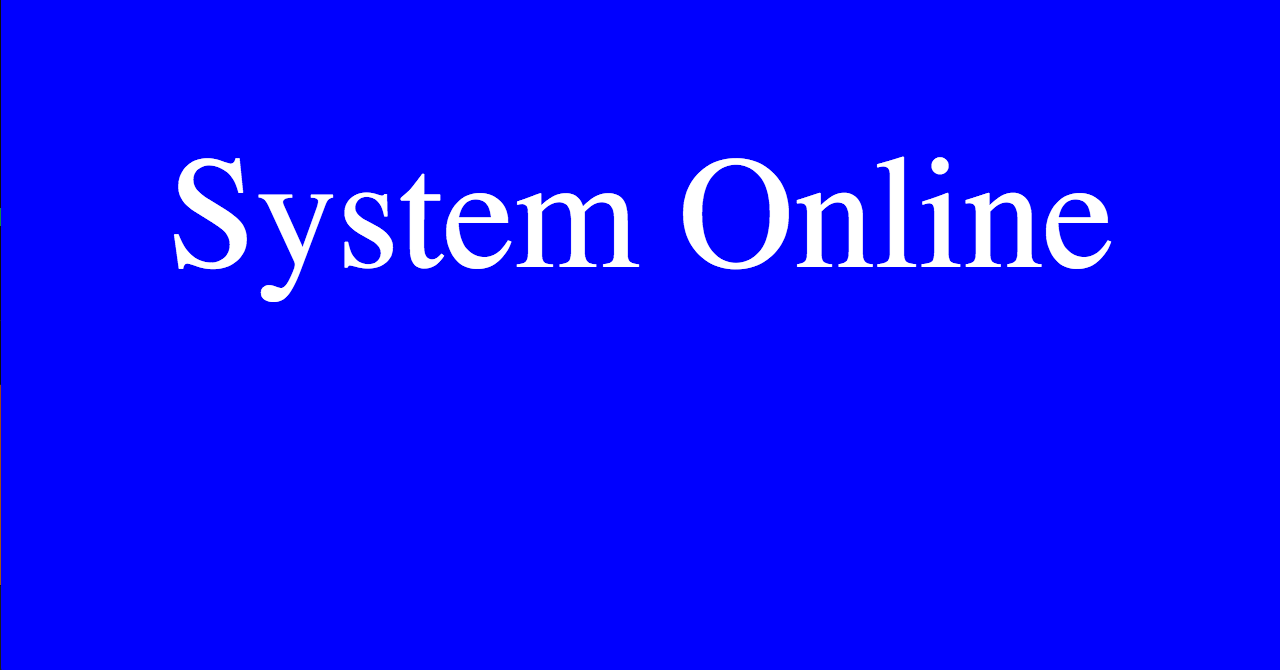
\includegraphics[width=\textwidth]{pics/state1}
                \caption{Online.}
                \label{fig:state1}
        \end{subfigure}
        ~
        \begin{subfigure}{0.45\textwidth}
                
\includegraphics[width=\textwidth]{pics/state2}
                \caption{Known caller.}
                \label{fig:state2}
        \end{subfigure}
		\\
		\begin{subfigure}{0.45\textwidth}
				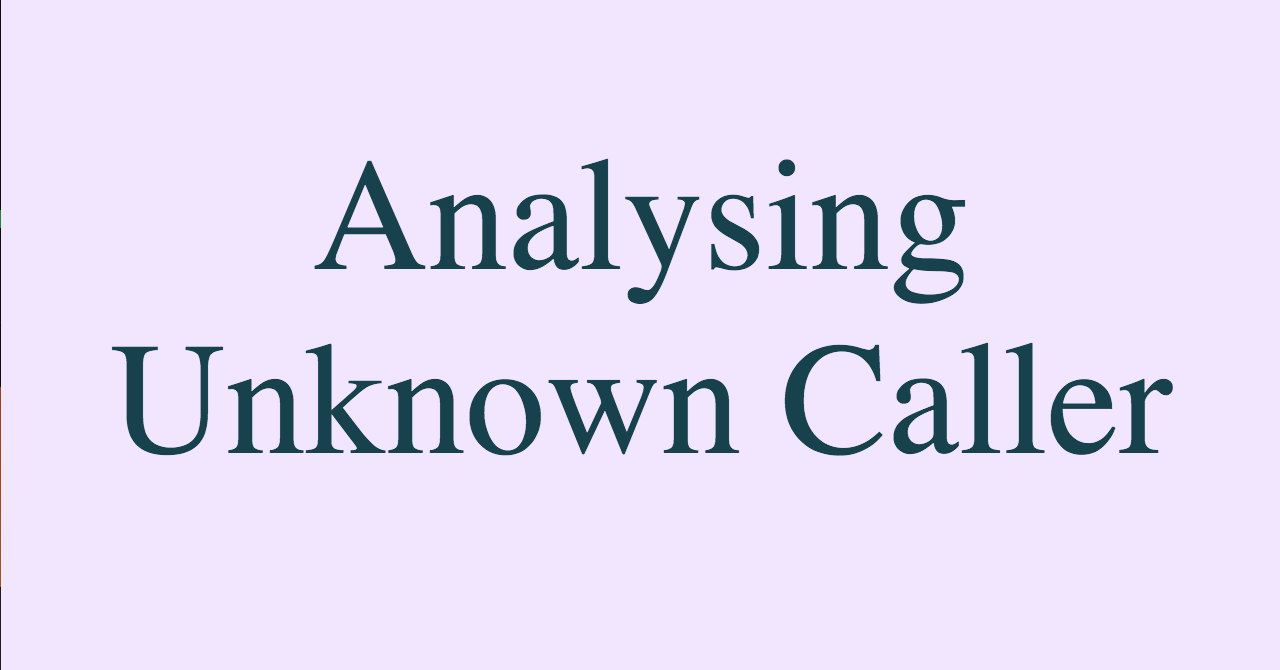
\includegraphics[width=\textwidth]{pics/state4}
				\caption{Voice analysis.}
				\label{fig:state4}
		\end{subfigure}
		~
		\begin{subfigure}{0.45\textwidth}
				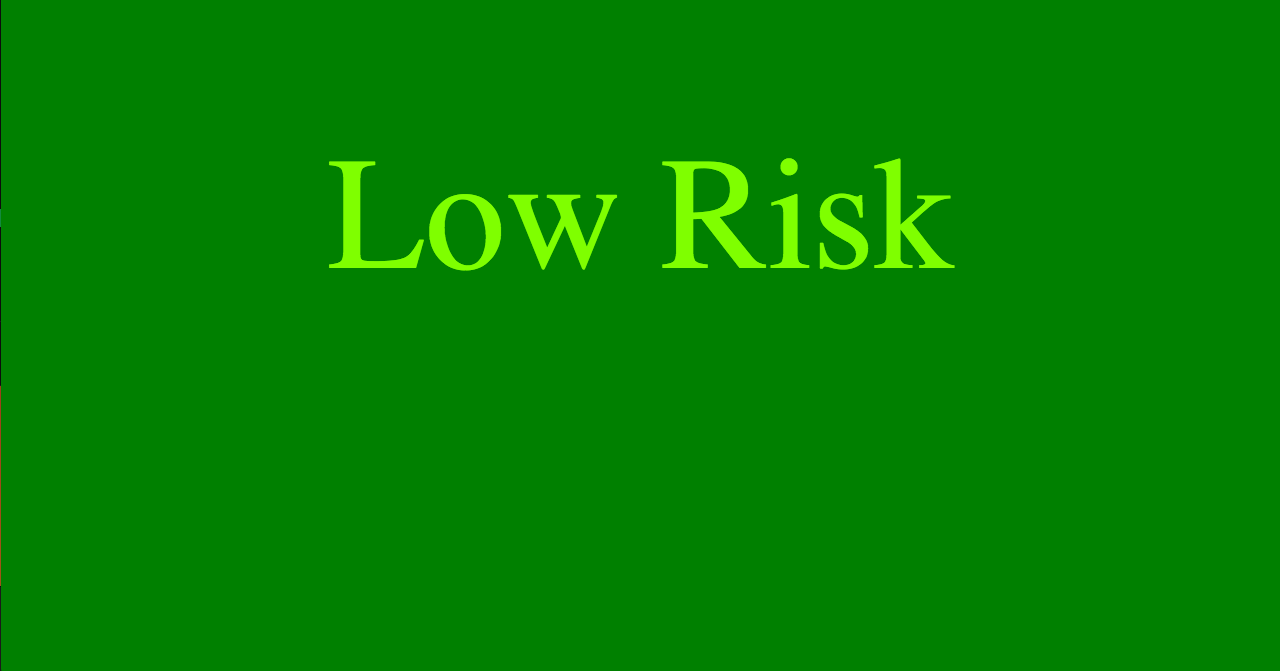
\includegraphics[width=\textwidth]{pics/state6}
				\caption{Low risk.}
				\label{fig:state6}
		\end{subfigure}
		\\
		\begin{subfigure}{0.45\textwidth}
				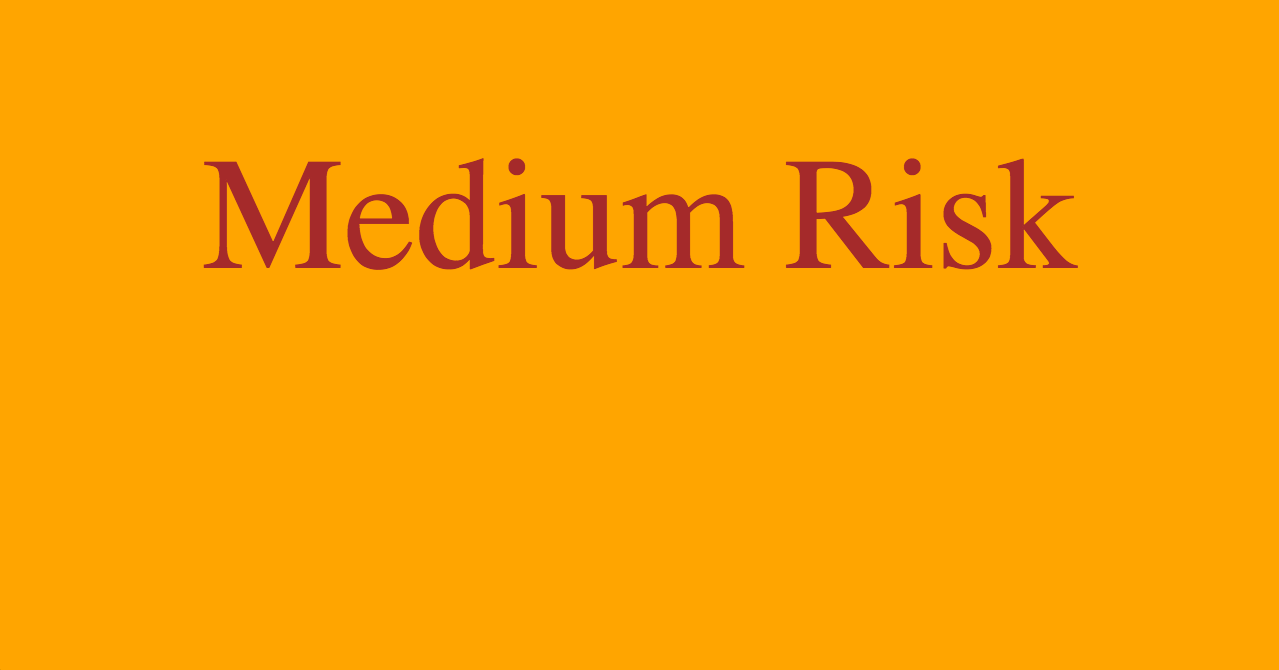
\includegraphics[width=\textwidth]{pics/state7}
				\caption{Medium risk.}
				\label{fig:state7}
		\end{subfigure}
		~
		\begin{subfigure}{0.45\textwidth}
				
\includegraphics[width=\textwidth]{pics/state8}
				\caption{High risk.}
				\label{fig:state8}
		\end{subfigure}
	\caption{Screens showing information to the user.}
	\label{fig:states}
\end{figure}

\section{Additional Components}
\subsection{Switch}
A switch was needed to determine the start and end of the call from the user's perspective. Introducing a bypass into the wires of the phone was not a good idea, as asking the user to make additional modifications was seen as undesirable. Instead, a physical switch was chosen, and it was one that was actuated by the handset being lifted off.
\\\\
The Raspberry Pi 3 offers GPIO inputs which allow digital inputs. To ensure that this was within the tolerances, a circuit powered by the Raspberry Pi's 3.3V output was designed. In Figure \ref{fig:initial-circuit} shows the layout. When the switch is closed, the GPIO pin reads the 3.3V from rail. When it is opened, the pin reads the voltage across the resistor.
\\\\
The Light Emitting Diode (LED) was used both as a debugging signal, and as a check for the user to ensure that installing the switch on their phone was done correctly. The LED was generously donated by Thomas Akinola, and was rated as having a 2V drop and recommended at 10mA. Knowing this, Equation \ref{eq:circuit} calculates the ideal resistor value. However, this caused the LED to be too bright, and a greater resistor value was chosen, $300\Omega$.
\vspace{-0.25cm}
\begin{align}
	\text{Resistor Value} &= \frac{\text{Voltage across Resistor}}{\text{Amperage needed}}\notag\\
	&= \frac{3.3\text{V} - 2\text{V}}{10\text{mA}}\notag\\
	&= \frac{1.3\text{V}}{10\text{mA}}\notag\\
	&\approx 130\Omega\label{eq:circuit}
\end{align}
\vspace{-1cm}

\begin{figure}[htb]
	\centering
	\begin{circuitikz} \draw
		 (0, 0) -- (8, 0)
		 (5, 0) to [R, l_=$300\Omega$] (5, 2)
		 (1, 2) node[label={above:To GPIO}] {} -- (5, 2)
		 (5, 4) to [led] (5, 2)
		 (3, 4) to [push button] (3, 2)
		 (0, 4) node[label={above:3.3V}] {} -- (8, 4)
		 (7, 0) node[ground]{} -- (7, 0)
		;
	\end{circuitikz}
	\caption{Initial switch circuit.} \label{fig:initial-circuit}
\end{figure}
\vspace{-0.5cm}

\subsection{Emergency Bypass}
The Obi110 suffers from a drawback in that it is powered from the mains. In a power cut, or emergency, the entire system would fail, and the phone would not be able to work. This is despite the fact that the phone lines are powered independently \cite{telephone}. Also, in an emergency, the system could be a serious liability. To prevent this, ideally, there should be an emergency bypass that can connect the phone directly to the landline. It would look like the setup in Figure \ref{fig:bypass}.

\begin{figure}[htb]
\centering
	\begin{tikzpicture}[node distance=3cm]
	    % We start by placing the blocks
	    \node [input, align=center] (input) {Input\\from\\Landline};
		\node [block, align=center, right of=input] (system) {The\\System};
		\node [output, align=center, right of=system] (output) {To\\Phone};
		\node [block, align=center, below of=system] (bypass) {Override\\Bypass};

	    % Once the nodes are placed, connecting them is easy.
	    \draw [draw,->] (input) -- node[align=center, name=in] {} (system);
	    \draw [->] (system) -- node[align=center, name=out]  {} (output);
		\draw [->] (input) |- node[align=center] {} (bypass);
		\draw [->] (bypass) -| node[align=center] {} (output);

	\end{tikzpicture}
	\caption{Emergency Bypass Visualisation}
	\label{fig:bypass}
\end{figure}

\end{document}
